\documentclass[11pt]{article}
\usepackage{weekly}
\begin{document}
\weekheader{4}{23/06 \textendash{} 30/06/2026}{Bộ nhớ hội thoại, Định vị cơ quan (bản đồ) và Đánh giá định lượng}{w4col}{Đã hoàn thành}

\section{Mục tiêu tuần}
Tuần cuối tập trung vào ba mảng để hoàn thiện trải nghiệm và kiểm chứng chất lượng hệ thống:
(1) trang bị bộ nhớ hội thoại đa lớp giúp trợ lý hỏi đáp đa lượt tự nhiên, giải được các tham
chiếu vượt cửa sổ lịch sử; (2) bổ sung tính năng định vị cơ quan xử lý thủ tục gần người dùng
kèm bản đồ và chỉ đường; (3) xây dựng bộ dữ liệu đánh giá có nhãn và đo định lượng toàn hệ
thống. Song song, nhóm hoàn thiện báo cáo chính và bốn báo cáo tuần.

\section{Công việc đã thực hiện}

\paragraph{Bộ nhớ hội thoại hai lớp (Conversation Memory): }
Tác tử ReAct ở pha gom nguồn vốn không dùng lịch sử hội thoại, nên các câu hỏi tiếp nối nằm
ngoài cửa sổ lịch sử dễ bị lạc chủ đề. Nhóm bổ sung một bộ nhớ phân tầng (\texttt{rag/memory.py})
đóng khung theo mô hình bộ nhớ kiểu hệ điều hành (MemGPT). \emph{Lớp A — Summary-Buffer} giữ
nguyên văn vài lượt gần nhất và tóm tắt bằng LLM các lượt cũ, qua đó giữ ngữ cảnh dài mà không
phình token. \emph{Lớp B — Episodic} lưu mỗi lượt hỏi đáp (và tuỳ chọn các \emph{fact} của
người dùng) vào một collection Chroma riêng, khoá theo \texttt{user\_id}, rồi truy hồi (recall)
top-$k$ ký ức liên quan trước khi tra cứu. Trước Giai đoạn 1, hệ tóm tắt và recall ký ức rồi
tiêm vào bước contextualize để viết lại câu hỏi tiếp nối thành câu hỏi độc lập --- ví dụ
``Lệ phí của thủ tục \emph{này} là bao nhiêu?'' được giải thành ``Lệ phí của thủ tục
\emph{xin cấp hộ chiếu phổ thông} là bao nhiêu?''. Sau mỗi lượt, cặp hỏi đáp được ghi vào ký
ức dài hạn. Mọi điểm gọi bộ nhớ đều được bọc \texttt{try/except} để lỗi bộ nhớ không bao giờ
làm hỏng câu trả lời; từng lớp bật tắt độc lập qua biến môi trường (\texttt{MEM\_SUMMARY},
\texttt{MEM\_EPISODIC}, \texttt{MEM\_FACTS}) phục vụ thí nghiệm cắt bỏ (ablation).

\screenshotfig{img/week4-memory.png}{Bộ nhớ episodic: câu hỏi tiếp nối kiểu ``thủ tục này''
được giải tham chiếu đúng nhờ ký ức của hội thoại trước.}{Bộ nhớ hội thoại giải tham chiếu đa
lượt.}{fig:w4-memory}

\paragraph{Định vị cơ quan xử lý thủ tục và bản đồ (Map): }
Sau khi nhận câu trả lời về một thủ tục, người dùng có thể bấm ``Địa điểm xử lý gần bạn'' để
tìm cơ quan, đơn vị tiếp nhận thủ tục gần vị trí hiện tại. Đây là tính năng do giao diện điều
phối, có endpoint dữ liệu ở backend (\texttt{rag/places.py}), không phải một công cụ trong
vòng lặp ReAct: vị trí đến từ trình duyệt và đầu ra là bản đồ tương tác. Luồng gồm bốn bước
(Hình~\ref{fig:w4-map}): lấy vị trí bằng định vị trình duyệt, hoặc nhập địa chỉ rồi geocode
bằng OpenStreetMap Nominatim khi bị từ chối; gọi SerpAPI (engine \texttt{google\_maps}) theo
chiến lược thích nghi theo khoảng cách (thử các mức zoom khác nhau, thêm hậu tố ``gần đây'' khi
truy vấn thưa), chuẩn hoá kết quả và sắp xếp theo khoảng cách haversine; hiển thị danh sách kèm
địa chỉ, số điện thoại, giờ làm việc, đánh giá và khoảng cách; vẽ bản đồ Leaflet trên nền
OpenStreetMap, tính tuyến đường bằng OSRM kèm quãng đường và thời gian lái xe ước tính, đồng
thời cung cấp liên kết mở Google Maps để điều hướng thật. Khi SerpAPI không có dữ liệu tại địa
bàn, hệ tự bổ sung kết quả web (Brave) dưới dạng thẻ tham khảo gắn nhãn chưa thẩm định. Các
dịch vụ dùng đều miễn phí và chỉ được gọi khi người dùng chủ động bấm.

\begin{figure}[H]
\centering
\resizebox{\textwidth}{!}{%
\begin{tikzpicture}[node distance=0.6cm and 0.8cm]
  \node[gbox] (loc)  {Vị trí người dùng\\(định vị / địa chỉ)};
  \node[fbox, right=of loc]  (serp) {SerpAPI Maps\\(thích nghi K.cách)};
  \node[fbox, right=of serp] (norm) {Chuẩn hoá\\+ sắp theo K.cách};
  \node[dbox, right=of norm] (list) {Danh sách cơ quan\\(địa chỉ, SĐT, giờ)};
  \node[abox, right=of list] (map)  {Bản đồ Leaflet\\+ tuyến OSRM};
  \draw[farr] (loc)--(serp); \draw[farr] (serp)--(norm);
  \draw[farr] (norm)--(list); \draw[farr] (list)--(map);
  \draw[farr, dashed] (serp.north) to[out=90,in=90]
        node[flab,above]{thiếu data: dự phòng web (Brave)} (list.north);
\end{tikzpicture}}
\caption{Luồng định vị cơ quan xử lý thủ tục và bản đồ chỉ đường.}
\label{fig:w4-map}
\end{figure}

\begin{figure}[H]\centering
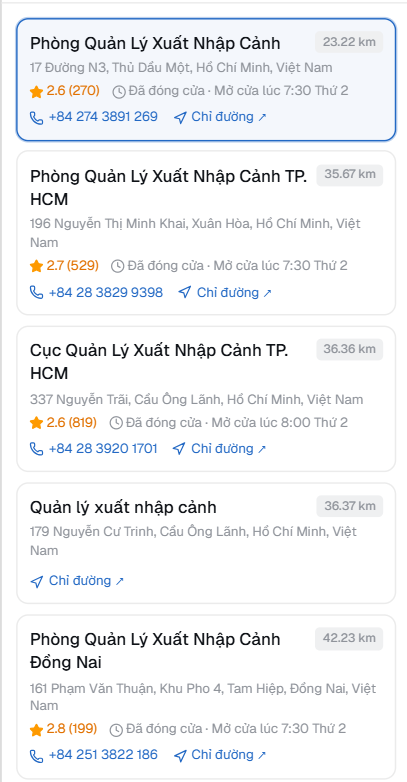
\includegraphics[width=0.42\textwidth]{img/week4-places-list.png}
\caption{Danh sách địa điểm xử lý gần người dùng: tên, địa chỉ, khoảng cách, đánh giá, sắp
xếp gần đến xa.}\label{fig:w4-places}
\end{figure}

\screenshotfig{img/week4-directions.png}{Bản đồ Leaflet và tuyến đường (OSRM) từ vị trí người
dùng tới cơ quan được chọn, kèm quãng đường và thời gian lái xe.}{Bản đồ và chỉ đường tới cơ
quan xử lý thủ tục.}{fig:w4-directions}

\paragraph{Thực nghiệm: đánh giá tầng sinh và trích dẫn: }
Tiếp nối đánh giá truy hồi ở tuần 3 (Hit@5 = 0,922), tuần này nhóm đo tầng sinh câu trả lời và
trích dẫn theo quy trình hai bước (bộ script \texttt{rag/eval/*}, kết quả lưu tại
\texttt{data/eval/}). Trước hết, chạy pipeline ReAct đầy đủ trên một tập con gồm 56 câu in-scope
(bảy nhóm $\times$ 8) và 8 câu ngoài phạm vi, lưu lại bộ (câu hỏi, câu trả lời, ngữ cảnh, trích
dẫn) làm cache để không phải sinh lại. Sau đó chấm bằng gpt-4o làm giám khảo theo hướng
reference-free (đối chiếu với chính bằng chứng và câu hỏi, không cần đáp án mẫu) trên các nhóm
độ đo: RAG Triad (faithfulness, answer relevance, context precision) theo họ TruLens; trích dẫn
theo ALCE (citation recall, precision, F1 dựa trên entailment giữa câu và nguồn dẫn); độ hoàn
chỉnh dựa trên checklist gold trích từ corpus; và abstention theo tinh thần SQuAD~2.0 (đo khả
năng từ chối câu ngoài phạm vi ở tầng câu trả lời).

\paragraph{Thực nghiệm: ablation bộ nhớ: }
Để tách riêng đóng góp của bộ nhớ, nhóm mô phỏng cửa sổ lịch sử ngắn (chỉ giữ 2 lượt gần nhất)
và đo độ chính xác giải tham chiếu --- câu hỏi tiếp nối sau khi viết lại có chứa đúng thực thể
của thủ tục đang nói tới hay không --- khi bật/tắt từng lớp. Phép thử B1 kiểm Lớp A
(Summary-Buffer) với tham chiếu nằm ở lượt cũ đã trôi khỏi cửa sổ; phép thử B2 kiểm Lớp B
(Episodic) với bối cảnh nằm ở hội thoại trước trong khi lịch sử hiện tại rỗng. Kết quả tổng hợp
ở Bảng~\ref{tab:w4-eval}.

\begin{table}[H]
\centering\small
\renewcommand{\arraystretch}{1.2}
\begin{tabular}{@{}llr@{}}
\toprule
Cụm & Chỉ số & Giá trị \\
\midrule
Sinh (n=56) & Faithfulness / Answer Relevance & 0,897 / 0,750 \\
            & Context Precision & 0,227 \\
Trích dẫn & Citation F1 (Recall / Precision) & 0,733 (0,742 / 0,725) \\
Hoàn chỉnh & Context Recall / Answer Completeness & 0,556 / 0,529 \\
Abstention & OOS từ chối / In-scope trả lời & 1,000 / 0,964 \\
\midrule
Bộ nhớ B1 (Lớp A) & Giải tham chiếu: không / có & 0\% / 100\% (n=4) \\
Bộ nhớ B2 (Lớp B) & Giải tham chiếu: không / có & 0\% / 100\% (n=3) \\
\bottomrule
\end{tabular}
\caption{Đánh giá tầng sinh, trích dẫn và ablation bộ nhớ (chi tiết trong báo cáo chính).}
\label{tab:w4-eval}
\end{table}

\noindent Faithfulness 0,90 cho thấy câu trả lời bám nguồn tốt, rủi ro ảo giác thấp; citation
F1 0,73 cho thấy trích dẫn đáng tin ở mức khá. Hệ từ chối đúng 100\% câu ngoài phạm vi mà gần
như không từ chối nhầm (in-scope answer 0,964). Context precision thấp (0,227) là chủ đích thiết
kế do cơ chế kéo đủ mọi mục của thủ tục, không phải lỗi truy hồi. Với bộ nhớ, cả B1 và B2 đều
cải thiện từ 0\% lên 100\%: khi tham chiếu vượt cửa sổ lịch sử, baseline viết lại sai hoàn toàn
còn bật bộ nhớ thì khôi phục đúng thực thể; cỡ mẫu nhỏ (n=4 và n=3) nên đây là minh chứng có
kiểm soát.

\paragraph{Hoàn thiện vận hành và báo cáo: }
Nhóm chuẩn hoá các kịch bản khởi chạy (\texttt{run-backend}, \texttt{run-frontend}) bật sẵn chế
độ UTF-8 để tránh lỗi mã hoá tiếng Việt trên console Windows, cùng cơ chế chia sẻ index dựng
sẵn qua HuggingFace để tái lập nhanh trên máy mới. Tầng LLM và embedding được cấu hình qua tệp
\texttt{.env} và trang Settings (hiện dùng Azure OpenAI \texttt{gpt-4o} và
\texttt{text-embedding-3-large}; có thể trỏ tới endpoint tương thích OpenAI), không phải sửa mã
nguồn. Về tài liệu, nhóm hoàn thiện báo cáo chính và bốn báo cáo tuần, thống nhất bốn sơ đồ
kiến trúc/pipeline và bảng số liệu giữa các tài liệu.

\section{Kết quả và sản phẩm bàn giao}
\begin{table}[H]
\centering\small
\begin{tabular}{@{}lp{8.7cm}@{}}
\toprule
Thành phần & Mô tả \\
\midrule
\texttt{rag/memory.py} & Bộ nhớ hội thoại 2 lớp: Summary-Buffer và Episodic (Chroma); ablation qua biến môi trường. \\
\texttt{rag/places.py}, \texttt{app/api/routers/places.py} & Endpoint định vị cơ quan: SerpAPI Maps thích nghi, haversine, dự phòng web. \\
\texttt{frontend/} (PlacesDialog, MapView) & Giao diện danh sách địa điểm + bản đồ Leaflet + tuyến đường OSRM. \\
\texttt{rag/eval/*}, \texttt{data/eval/*} & Bộ script và kết quả ba thí nghiệm đánh giá định lượng. \\
Bộ báo cáo PDF & Báo cáo chính, bốn báo cáo tuần và bốn sơ đồ kiến trúc/pipeline. \\
\bottomrule
\end{tabular}
\end{table}

\section{Khó khăn và hướng xử lý}
\begin{itemize}
  \item Bộ nhớ episodic dùng Chroma cần đường dẫn ASCII để tránh lỗi ghi tệp nhị phân của
        hnswlib trên Windows; khi chưa có xác thực, \texttt{user\_id} tạm cố định là
        \texttt{default}.
  \item Định vị trình duyệt yêu cầu \texttt{localhost} hoặc HTTPS, và trên máy không có Wi-Fi
        thường không lấy được toạ độ chính xác: hệ có sẵn lối nhập địa chỉ tay (geocode bằng
        Nominatim) làm phương án chắc chắn.
  \item Hạn mức và độ ổn định dịch vụ ngoài: SerpAPI gói miễn phí chỉ khoảng 100 lượt mỗi
        tháng nên tính năng chỉ gọi khi người dùng bấm; OSRM và Nominatim công cộng không có
        SLA, phù hợp demo chứ chưa phải production.
  \item Quy mô đánh giá còn vừa (đặc biệt ablation bộ nhớ với cỡ mẫu nhỏ) và phần lớn dùng LLM
        làm giám khảo: nhóm nêu rõ giới hạn và xem human evaluation quy mô lớn là hướng tiếp theo.
\end{itemize}

\section{Checklist tuần 4}
\begin{itemize}[label={}]
  \cbDone Bộ nhớ hội thoại 2 lớp (Summary-Buffer + Episodic Chroma), ablation qua biến môi trường.
  \cbDone Tính năng định vị cơ quan xử lý + bản đồ Leaflet + chỉ đường OSRM + dự phòng web.
  \cbDone Thực nghiệm đánh giá tầng sinh, trích dẫn và ablation bộ nhớ (tiếp nối đánh giá truy hồi ở tuần 3).
  \cbDone Hoàn thiện báo cáo chính, bốn báo cáo tuần và bốn sơ đồ kiến trúc/pipeline.
\end{itemize}

\section{Kết luận dự án}
Sau bốn tuần, đồ án đi trọn một vòng từ khâu dữ liệu (5.208 thủ tục, kho truy hồi ba lớp), qua
đường cơ sở một lượt có trích dẫn, tới kiến trúc Agentic RAG (tác tử ReAct hai giai đoạn có
minh bạch hoá suy luận và trích dẫn kèm tô sáng), và cuối cùng là bộ nhớ hội thoại đa lượt,
tính năng định vị cơ quan xử lý kèm bản đồ chỉ đường, cùng đánh giá định lượng toàn hệ thống.
Kết quả là một trợ lý hỏi đáp thủ tục hành chính công có căn cứ, minh bạch, hỏi đáp đa lượt và
đã được kiểm chứng định lượng.

\end{document}
